\documentclass[12pt]{article}
%\usepackage{makeidx}
%\usepackage{multirow}
%\usepackage{multicol}
%\usepackage[dvipsnames,svgnames,table]{xcolor}
%\usepackage{graphicx}
%\usepackage{epstopdf}
%\usepackage{ulem}
%\usepackage{hyperref}
%\usepackage{amsmath}
%\usepackage{amssymb}

\usepackage[sorting=none]{biblatex}
\usepackage[french]{babel}
\usepackage[T1]{fontenc}
\usepackage{float}
\usepackage{graphicx}
\usepackage[utf8]{inputenc} 
\usepackage{csquotes}
\usepackage{pdfpages}
\usepackage{url}

\addbibresource{webographie.bib}

\title{Rapport de stage}
\usepackage[paperwidth=595pt,paperheight=841pt,top=56pt,right=56pt,bottom=56pt,left=56pt]{geometry}

\makeatletter
	\newenvironment{indentation}[3]%
	{\par\setlength{\parindent}{#3}
	\setlength{\leftmargin}{#1}       \setlength{\rightmargin}{#2}%
	\advance\linewidth -\leftmargin       \advance\linewidth -\rightmargin%
	\advance\@totalleftmargin\leftmargin  \@setpar{{\@@par}}%
	\parshape 1\@totalleftmargin \linewidth\ignorespaces}{\par}%
\makeatother 

% new LaTeX commands
\parindent=5pt

\begin{document}


\begin{center}

\vspace{3pt} \noindent
\begin{tabular}{p{439pt}}
\parbox{439pt}{\centering 
\includegraphics[width=125pt]{gallery/img-3.png}\textbf{{\large 

\includegraphics[width=146pt]{gallery/img-2.png}
}}
\includegraphics[width=132pt]{gallery/img-1.png}{\small  }} \\

$ $

\parbox{439pt}{\centering 
{\Huge Rapport de stage 2A}
} \\
\hline
\parbox{439pt}{\centering 
\textit{{\Huge Menou Camille}}
} \\
\parbox{439pt}{\centering } \\
\parbox{439pt}{\centering 
\textbf{\textit{{\Large Camille Menou}}}
} \\
\parbox{439pt}{\centering } \\
\end{tabular}
\vspace{2pt}

\end{center}



\begin{center}
\textbf{Ann\'{e}e 2016-2017}
\end{center}

\begin{center}
Stage de 2$^{e}$ année réalisé dans l'équipe \textit{COAST}
\end{center}

\begin{center}
\textit{Logo de l'entreprise}
\end{center}

{\raggedright
Maître de stage~: \textit{Philippe Kalitine}
\\
Encadrant universitaire~: \textit{Alexandre Parodi}\pagebreak{}
}

\begin{center}
\textbf{{\huge Déclaration sur l'honneur de non-plagiat}}
\thispagestyle{empty}
\end{center}

$ $

\textbf{Je soussignée,}

\textbf{Menou Camille}

\textbf{\'{E}lève-ingénieure régulièrement inscrite en 2$^{e}$
année à TELECOM Nancy}

\textbf{N$^\circ{}$ de carte d'étudiant(e)~:} 13538235

\textbf{Année universitaire~:} 2016 - 2017

\textbf{Auteur(e) du document, m\'{e}moire, rapport ou code informatique
intitul\'{e}~: Rapport de stage 2A}

$ $


Par la présente, je déclare m'être informée sur les
différentes formes de plagiat existantes et sur les techniques et normes de
citation et référence.

Je déclare en outre que le travail rendu est un travail original, issu de ma
réflexion personnelle, et qu'il a été rédigé entièrement
par mes soins. J'affirme n'avoir ni contrefait, ni falsifié, ni copié
tout ou partie de l'\oe{}uvre d'autrui, en particulier texte ou code
informatique, dans le but de me l'accaparer.

Je certifie donc que toutes formulations, idées, recherches, raisonnements,
analyses, programmes, schémas ou autre créations, figurant dans le
document et empruntés à un tiers, sont clairement signalés comme
tels, selon les usages en vigueur.

Je suis consciente que le fait de ne pas citer une source ou de ne pas la
citer clairement et complètement est constitutif de plagiat, que le plagiat est
considéré comme une faute grave au sein de l'Université, et qu'en cas
de manquement aux règles en la matière, j'encourrais des poursuites non
seulement devant la commission de discipline de l'établissement mais
également devant les tribunaux de la République Française.

\begin{center}
\textbf{Fait à Villers-lès-Nancy, le unjour/08/2017}
\end{center}
\thispagestyle{empty}

\begin{center}
\textbf{Signature~:}
\end{center}

\newpage
\thispagestyle{empty}
\section*{Résumé :}
Coming soon...

\section*{Abstract :}
Coming soon...


%Pour insérer une image facilement :
%\begin{figure}[H]
%\centering
%\includegraphics[scale=0.4]{fichier de l'image}
%\caption[nom dans le sommaire]{légende}
%\label{fig:gallery}
%\end{figure}

\newpage
\thispagestyle{empty}
\section*{Remerciements}
Mes tout premiers remerciements sont adressés à M. Philippe Kalitine, ingénieur de recherche chez COAST et mon maître de stage. Merci pour la confiance, l'indépendance et l'expertise qui m'ont permises de mener à bien les tâches qui m'étaient confiées.\\

Merci à TELECOM Nancy pour la mise en place de cette période de stage afin que ses étudiants de seconde année puissent acquérir une expérience technique indispensable à la formation d'un ingénieur.\\

Merci à mon encadrant universitaire, M. Alexandre Parodi pour la supervision de ce stage et la lecture et notation de ce rapport.\\

De manière générale merci à toute l'équipe COAST pour sa convivialité. Venir travailler avec vous ce n'était plus du travail, mais l'exercice d'une passion commune dans une excellente ambiance !\\

Enfin, je tiens à remercier toutes les personnes qui se sont donnés la peine de relire ce rapport : Coming soon.

\newpage
\thispagestyle{empty}
\tableofcontents

\newpage
\setcounter{page}{1}
\addcontentsline{toc}{section}{Introduction}
\section*{Introduction}
Dans le cadre de ma deuxième année dans l'école d'ingénieur TELECOM Nancy, j'ai effectué un stage technicien au Laboratoire lorrain de recherche en informatique et ses applications (LORIA) \cite{loria} à Villers-lès-Nancy. Durant dix semaines j'ai travaillé au sein de l'équipe COAST \cite{coast} dirigée par François Charoy, du 6 juin au 11 août de l'année 2017. Ce stage m'a été proposé par Philippe Kalitine, ingénieur en recherche en informatique chez COAST.\\

L'équipe travaille actuellement sur MUTE \cite{mute}, un éditeur web de texte collaboratif pair-à-pair open source (comprendre une application comme Google Doc mais sans avoir à stocker le document sur un serveur) qui a pour vocation de devenir l'éditeur de texte principal du personnel Inria \cite{inria}.\\

L'objectif de mon stage était de rendre l'éditeur riche, par exemple en intégrant des fonctionnalités autour de l'ajout de style dans les documents, d'images, de formules mathématiques, ou bien autour de l'exportation dans divers formats (PDF, HTML, etc.).\\

Dans le contexte de ce stage qui est celui de la recherche, il y a moins la pression d'une deadline, comme on le voit en entreprise. Cependant l'équipe COAST se prépare à faire une démonstration de MUTE lors de la quinzième European Conference on Computer-Supported Cooperative Work (ECSCW) \cite{ecscw} et qui aura lieu du 28 août au 1er septembre 2017 à Sheffield (UK). L'enjeu n'était donc pas des moindres et suggérait un travail de qualité.\\

Ce document constitue le rapport de ce stage. Dans un premier temps, nous poserons le contexte en parlant de l'équipe COAST au sein du LORIA et de ces objectifs. S'ensuivront une mise en lumière de l'origine du projet ainsi que les objectifs du stage. Nous détaillerons ensuite l'ensemble des développements mis en place, les résultats obtenus et les difficultés rencontrées. Enfin, nous dresserons un bilan de cette expérience technique en laboratoire de recherche et parlerons d'éventuelles améliorations à apporter au projet.\\

\newpage
\section{L'équipe COAST, INRIA : présentation}
\subsection{COAST}
\subsubsection{LORIA}
Coming soon...
\subsubsection{INRIA}
Coming soon...
\subsubsection{L'équipe COAST}
Coming soon...

\subsection{Organigramme du LORIA et de COAST}
Coming soon...

\newpage
\section{Problématique du stage : rendre un éditeur de texte riche}
\subsection{Mise en contexte : MUTE}
\paragraph{Origine du besoin}
A l'heure actuelle, au sein des entreprises, l'édition et le partage de fichiers entre collègues se fait très souvent sous forme de mail où le fichier est mis en pièce jointe. Cette pratique est très contraignante pour plusieurs raisons :\\
\begin{itemize}
    \item c'est une procédure chronophage.
    \item les modifications apportées ne sont pas évidentes à voir.
    \item si beaucoup de personnes doivent modifier le même document et plus précisément un même paragraphe, la fusion de ces modifications devient très laborieuse.
    \item l'envoi d'un mail contenant des rapports confidentiels expose l'entreprise à des espionnages industriels.
\end{itemize}
\paragraph{}
Pour pallier ce problème, certains proposeraient tout simplement d'utiliser Google Doc, l'éditeur de texte de Google, qui a l'avantage d'apporter une édition collaborative d'un document et en temps-réel. Malheureusement, Google Doc utilise une architecture dite, centralisée : un serveur stocke le document et écoute les modifications des collaborateurs. De cela découlent trois inconvénients majeurs empêchant la mise en place de cette solution en entreprise :\\
\begin{itemize}
    \item l'utilisation de l'éditeur devient difficile à gérer pour le serveur à partir d'une quinzaine personnes.
    \item le fait que le document soit stocké sur les serveurs de Google ne plaît pas aux entreprises pour une question de sécurité (vol de données) mais aussi de sûreté (la sauvegarde du document peut être compromise si les serveurs de Google subissent une panne).
    \item l'édition d'un document devient impossible si les serveurs de Google sont en difficulté ou si notre connexion internet devient instable.
\end{itemize}
\paragraph{}
Afin de développer une plate-forme collaborative permettant de répondre à ces besoins, le projet OpenPaaS \cite{openpaas} a été créé. Financé par BpiFrance \cite{bpi}, les sociétés Linagora \cite{linagora}, XWiki SAS \cite{xwiki}, Nexedi \cite{nexedi} et le laboratoire d'informatique de l'école polytechnique ont collaboré à ce projet open-source français.
\paragraph{}
A cette intention, l'expertise de l'équipe COAST a été requise. L'objectif principal qui leur était attribué : montrer qu'il est possible de mettre en place
\begin{itemize}
    \item un réseau pair-à-pair capable de mieux passer à l'échelle que Google Doc.
    \item une collaboration sûre (sans pertes de données).
\end{itemize}
\paragraph{}
COAST a donc créé l'API indépendante mute-core \cite{mute-core}, constituée de deux sous-projets :

\paragraph{Mute-structs}
Mute-structs \cite{mute-structs} est un projet Node.js qui propose une implémentation de l'algorithme CRDT (Conflict-free replicated data type) LogootSplit \cite{logoot}. Il est issu de la thèse de Luc André et sert à la fusion des contributions des collaborateurs sans générer de doublons ou de perte de données.

\paragraph{Netflux}
Nextflux \cite{netflux} est une API permettant l'établissement d'un réseau pair-à-pair, basée sur les technologies Web Real-Time Communication (WebRTC) et WebSocket. A l'origine, cette API se basait sur la topologie fully-connected \cite{fully} : si un réseau comporte n pairs, il existe n-1 liens pour relier tous les pairs entre eux. Mon camarade d'école Laurent Bidet et aussi en stage chez COAST a, lui, développé une topologie basée sur l'algorithme Spray \cite{spray}. Cette algorithme permet de réduire le nombre de liens à log(n).

\paragraph{MUTE}
L'équipe COAST a décidé de développer leur propre éditeur collaboratif afin qu'il soit utilisé au sein de l'INRIA, et, pourquoi pas, au sein de TELECOM Nancy, école d'ingénieur voisine du laboratoire et où j'étudie actuellement. Multi User Text Editor (MUTE) est donc une interface web basée sur l'API CodeMirror et qui se sert de l'API mute-core. MUTE est donc un éditeur web collaboratif temps-réel pair-à-pair.

\begin{figure}[H]
\centering
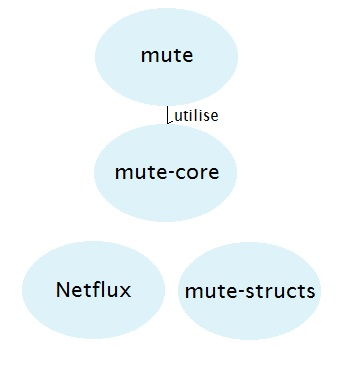
\includegraphics[scale=0.52]{gallery/hierarchy.jpg}
\caption[nom dans le sommaire]{Hiérarchie de mute-core, API utilisée par MUTE}
\label{fig:gallery0}
\end{figure}

\subsection{Description et analyse du problème posé : apporter une édition riche}
L'ensemble de mon travail portait sur le projet MUTE et consistait en du Front-End. L'objectif consistait en une amélioration de l'expérience utilisateur de MUTE.


\subsection{Cahier des charges}
Le cahier des charges du projet Rich Text Editor a été défini comme étant les issues GitHub auxquelles j'étais assignée. Les détails nécessaires m'ont été fournis à l'oral au moment opportun. Ci-dessous, la liste des issues que je devais réaliser pendant mon stage :\\

As a User I want to :
\begin{description}
    \item [see a partially styled (inline rendered style) Markdown text in the editor :]les balises correspondant à de la syntaxe Markdown doivent être camouflés après interprétation du style, une fois que l'édition du texte stylisé est terminée ou qu'on met le focus ailleurs. De même, les balises doivent réapparaître lorsque l'utilisateur met le focus sur un élément contenant du style.
    \item [see a rendered version of my document :]cette issue est devenue obsolète du fait de la précédente (voir explications dans la partie Réalisation et validation). Concrètement, si l'issue précédente n'était pas réalisable immédiatement, il aurait fallu compléter cette issue, étape intermédiaire entre ce qui existait au début du stage, et ce qui existe maintenant. L'idée était la suivante : MUTE aurait dû être divisée en deux parties : à gauche l'utilisateur écrirait le texte souhaité, à droite il aurait accès à un rendu où la syntaxe aurait été interprétée.
    \item [have an outline view for Markdown :] Coming soon...
    \item [add basic styles (bold, italic...) to the document using keyboard shortcuts :]l'utilisateur doit pouvoir ajouter/enlever du style en utilisant des raccourcis claviers intuitifs, par exemple Ctrl+B pour le gras.
    \item [add basic styles (bold, italic...) to the document using toolbar :]au moment d'une sélection de texte, une barre d'outils doit apparaître pour que l'utilisateur puisse ajouter/enlever le style à la souris.
    \item [see my math formula rendered :]l'utilisateur doit pouvoir écrire une formule mathématique et qu'elle ait le même rendu que s'il l'avait écrite à la main.
    \item [include images into my documents :]tout est dans l'intitulé.
    \item [to add some "End of Page" character :]au bout d'un certain nombre de lignes, la page doit se terminer et une nouvelle doit être créée.
    \item [consult Markdown cheat-sheet :]l'utilisateur doit pouvoir rapidement accéder à la syntaxe de Markdown
    \item [consult MathJax cheat-sheet :]l'utilisateur doit pouvoir rapidement accéder à la syntaxte de MathJax
    \item [be able to export the document to another document format (PDF, plain text) :]tout est dans l'intitulé.\\
\end{description}

Les issues à propos des cheat-sheets et de l'exportation comportaient le tag "optionnal" pour dénoter une priorité basse. Les autres issues ont été classées par ordre de priorité décroissante, comme ci-dessus.

L'ensemble de mon travail était régi par un besoin fonctionnel incontournable : si des fonctionnalités visent à modifier le contenu du document alors le contenu doit effectivement être modifié, et ce pour n'importe quel collaborateur du document. Un autre besoin, non négligeable, était que les développements marchent à la fois sur Chrome et sur Firefox.

\newpage
\section{Réalisation et validation}
\subsection{Auto-formation}
\paragraph{}
Le stage a d'abord commencé par une période d'auto-formation à base de Massive Open Online Courses (MOOCs), de vidéos de conférences et d'articles écrits par des développeurs/ingénieurs de la communauté informatique. A cette occasion, et pendant les onze premiers jours je me suis donc formée en JavaScript et en TypeScript (JavaScript typé).
\paragraph{}
Le projet utilisant le framework AngularJS j'ai également lu à ce sujet grâce au apparemment assez célèbre Tour of Heroes \cite{tour}, projet Angular écrit pour un tutoriel disponible sur le site officiel d'Angular \cite{angular}.

\subsection{Environnement de travail}
\paragraph{}
La partie édition de MUTE est basée sur une API qui s'appelle CodeMirror \cite{codemirror}. Il s'agit d'un éditeur de texte écrit en JavaScript et pensé pour les navigateurs. Ce projet assez populaire (12,364 stars et 3000 forks au 4 août 2017) est agrémenté d'addons très utiles rendant CodeMirror très polyvalent.

\paragraph{}
L'ensemble du projet est hébergé sur un répertoire GitHub, un gestionnaire de version.

\paragraph{}
Il m'a été conseillé d'utiliser VisualStudio Code pour développer. Particulièrement adapté au langage JavaScript, VisualStudio permet de voir très facilement les fichiers modifiés par rapport au dernier commit et de faire des merges très simplement.

\paragraph{}
Le projet utilise le framework Angular. (expliquer les components)

\paragraph{}
Pour gérer ses dépendances, le projet utilise npm \cite{npm}, un package manager.\\

(npm cz pour voir si le code est formaté correctement.)\\

(digest pour repérer des divergences.)\\

\subsection{Méthode de travail}
Deux outils m'ont quotidiennement aidée à m'organiser et à prendre des notes pour faciliter l'écriture de ce rapport : l'outil de gestion de projet GitHub, ainsi qu'un journal quotidien que j'ai tenu selon le principe du bullet journal \cite{bullet}.

\paragraph{GitHub workboard}
Je le nomme workboard car il se présente comme un tableau référençant l'ensemble des issues m'étant attribués, de la documentation et ma roadmap. En voici un aperçu :

\newpage
\begin{figure}[H]
\centering
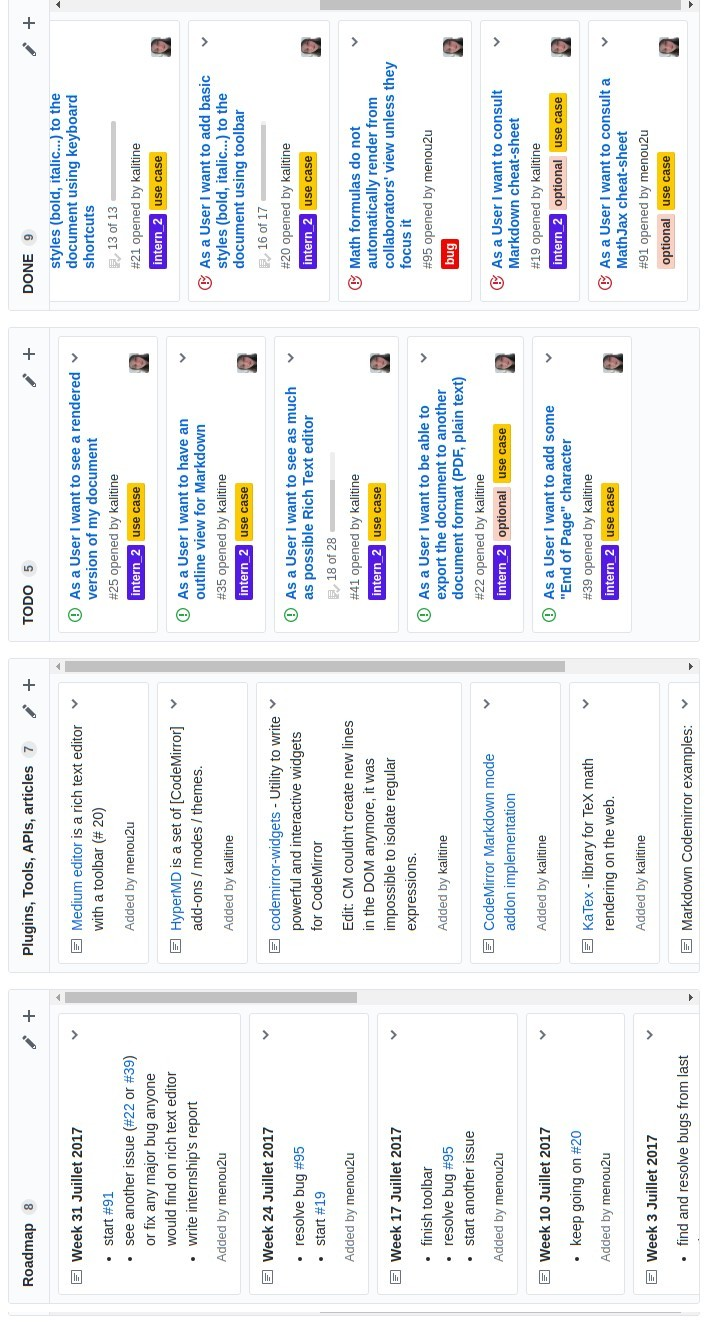
\includegraphics[scale=0.52]{gallery/workboard.jpg}
\caption[nom dans le sommaire]{Workboard du projet Rich Text Editor}
\label{fig:gallery1}
\end{figure}

\newpage
C'était également un excellent moyen pour accéder rapidement à mes issues et cela permettait également à mon maître de stage de pouvoir jeter un oeil à mon avancement. C'est une fonctionnalité de GitHub que je ne connaissais pas avant ce stage et qui se révèle être l'outil rêvé pour des fondus d'organisation.\\

\paragraph{Journal quotidien}
Afin de noter un maximum de choses pour écrire ce rapport mais aussi pour noter ma réflexion, ne pas oublier de faire quelque chose ou juste mieux m'organiser, j'ai pris l'initiative de tenir un journal quotidien de mon travail. A cette occasion j'ai repris quelques principes des bullet journals comme par exemple le fait de noter systématiquement les tâches à faire en organisant des checklists. Pour lier le workboard au journal, j'ai noté chaque jour sur quelle(s) issue(s) j'ai travaillé avec un code couleur pour retrouver plus rapidement des notes que j'aurais prises à l'intention de l'une d'elles.\\

\paragraph{Compléter une issue}
Avant de commencer une issue, j'en informais mon maître de stage qui me donnait certaines pistes de réflexion et de recherche à explorer avant de commencer.
\paragraph{}
Ainsi, en toute autonomie, je menais des recherches les plus exhaustives possibles pour trouver des solutions open source ou juste des méthodes que j'aurais pu reproduire dans notre projet. Nous voyions ensuite ensemble le meilleur choix.
\paragraph{}
Après le développement de la solution, je montrais le résultat, relevant les limites et recevant des détails à rajouter au développement. Pour certaines issues, notamment pour les raccourcis clavier et la barre d'outils, je référençais sur l'issue correspondante l'ensemble des fonctionnalités présentes. Voici un exemple :

\newpage
\begin{figure}[H]
\centering
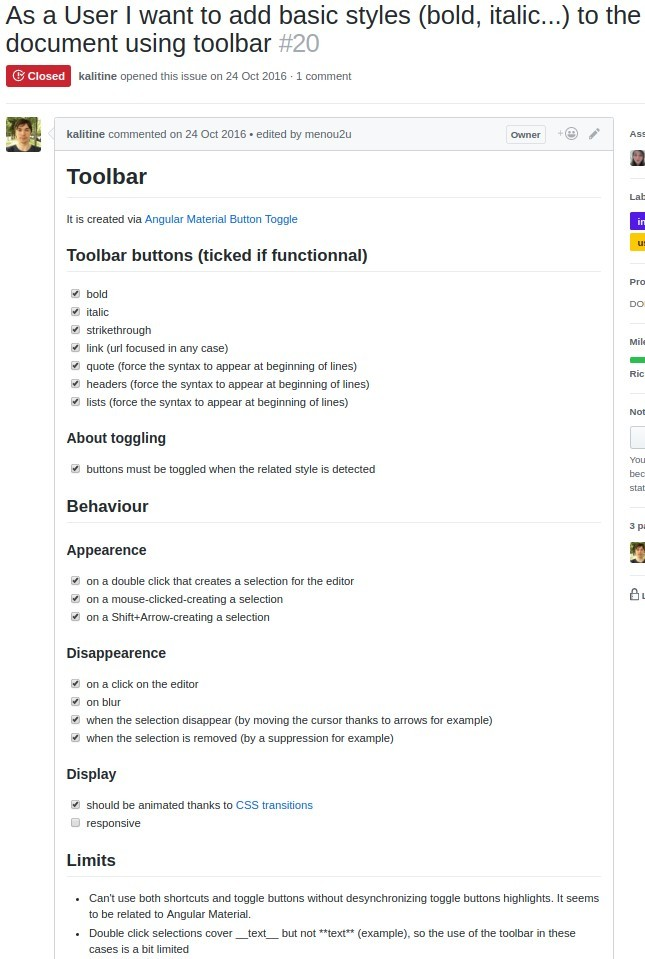
\includegraphics[scale=0.75]{gallery/issue.jpg}
\caption[nom dans le sommaire]{Issue associée à la barre d'outils}
\label{fig:gallery2}
\end{figure}
\newpage
L'avantage de cette pratique est qu'il sera possible pour les personnes qui maintiendront mon code de voir s'il y a eu des régressions ou tout simplement de voir ce qui existe déjà et ce qu'il reste à faire.\\

\paragraph{Communication avec l'équipe}
Lors des premières semaines, chaque vendredi 13h, l'équipe se réunissait pour faire état de l'avancement de chacun.
L'équipe utilise également Slack \cite{slack} pour communiquer.\\

\newpage
Abordons maintenant de manière plus concrète les différentes étapes de réalisation du cahier des charges.\\

\subsection{Cacher la syntaxe Markdown : intégration d'HyperMD}
Afin d'apporter du style à l'éditeur (gras, italique, etc.), l'équipe a décidé d'utiliser le langage à balise Markdown \cite{markdown}. A mon arrivée, MUTE était déjà configuré pour interpréter ce langage et l'on obtenait ce rendu :

\begin{figure}[H]
    \centering
    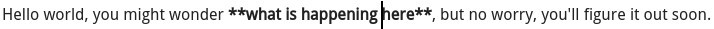
\includegraphics[scale=0.65]{gallery/style_example.jpg}
    \caption[nom dans le sommaire]{Syntaxe Markdown apparente}
    \label{fig:gallery3}
\end{figure}

L'on constate que le style est appliqué mais que les balises sont encore visibles. Comme indiqué dans le cahier des charges, l'une de mes tâches a été de faire en sorte de cacher la syntaxe.

\subsubsection{Premières approches}
\paragraph{Une approche à la main}
Il s'agissait de la première issue que j'avais à faire. Je n'avais pas encore à l'esprit l'importance de la contribution des gens dans le milieu open source. Car, encore une fois, CodeMirror est un projet assez populaire et le nombre de projets "dérivés" est important. Donc, dans un premier temps, j'ai essayé de résoudre le problème avec "les moyens du bord".
\paragraph{}
Dans mon analyse de la situation, j'ai remarqué que l'utilisation de la syntaxe Markdown au sein de l'éditeur modifiait le DOM \cite{dom}. Le DOM est une interface de programmation qui, entre autres, organise le contenu d'une page HTML en une structure d'arbre qu'il est possible de parcourir et modifier. Si on reprend l'exemple de l'image ci-dessus, on obtient le DOM suivant :
\begin{figure}[H]
    \centering
    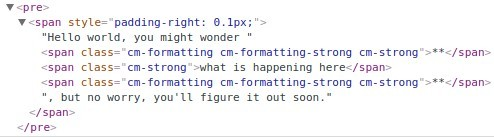
\includegraphics[scale=0.95]{gallery/modified_dom.jpg}
    \caption[nom dans le sommaire]{DOM modifié}
    \label{fig:gallery4}
\end{figure}
\paragraph{}
De ce fait, je pensais faire une recherche des noeuds du DOM dont les classes contiendraient des éléments en rapport avec le style CSS apporté par Markdown. Une fois ce style récupéré il aurait fallu l'appliquer uniquement au "what is happening here". Pour faire disparaître les balises sans pour autant les perdre, j'aurai essayé d'appliquer l'attribut CSS visibility en le mettant à "hidden" aux deux spans contenant les balises.
\paragraph{}
Cependant, cette solution paraissait trop lourde car elle nécessitait un parcours constant du document. De plus, si une personne avait été en train d'écrire, l'édition en aurait été gênée.

\paragraph{}
Mon maître de stage m'a alors suggéré de rechercher des API développées en ce sens à intégrer dans notre projet.

\paragraph{Une première API : codemirror-widgets}
Coming soon.\\
https://github.com/SamyPesse/codemirror-widgets


\subsubsection{HyperMD}
N'arrivant toujours pas à utiliser codemirror-widgets à nos fins, mon maître de stage m'a dirigée vers d'autres API, entre autres HyperMD \cite{hypermd}, projet datant de Janvier 2017, et dont la démo \cite{demo} paraissait remplir les objectifs de cette première issue et plus.
Après avoir installé HyperMD dans notre projet, nous avons constaté qu'en plus de cacher la syntaxe, les liens étaient stylisés, les images étaient prises en compte, ainsi que les formules mathématiques, grâce à MathJax \cite{mathjax}.\\

(parler du service)\\
(faudra introduire un peu MathJax ici, comment ça marcher viteuf (back et front), dire qu'on a repéré un bug)\\

J'ai pris l'initiative de créer une issue pour créer une cheat-sheet pour MathJax, à l'instar de Markdown, afin d'améliorer l'expérience utilisateur.\\

\newpage
\subsection{Modifier le style}
\subsubsection{Ajout de raccourcis clavier}
Coming soon...

\subsubsection{Création d'une barre d'outils}
(parler de Material Angular, expliquer qu'un module c'est un Component Angular)\\
(parler des guidelines angular)\\
(parler de la désynchro)\\
(cacher sur téléphone)\\
Coming soon...

\newpage
\subsection{Adaptation des appels à MathJax}
MathJax est une librairie offrant une grande diversité de symboles mathématiques. La manière dont HyperMD fait appel à cette librairie correspond parfaitement au besoin décrit dans le cahier des charges, mais ne répond pas à la notion de collaboration. La multitude de scénarios possible dans un contexte temps-réel collaboratif fait que j'ai dû me pencher sur le problème qui va suivre à plusieurs reprises. Il est d'ailleurs certains que des cas limites ne soient pas encore traités.

\subsubsection{Analyse de la situation}
\paragraph{}
Lors de l'intégration d'HyperMD au projet, j'ai remarqué que si un collaborateur A décidait de modifier une formule, un collaborateur B ne verrait le changement que s'il mettait le focus sur cette formule. Même si cela ne reste qu'un bug d'affichage ne causant pas de divergences, j'ai proposé à mon maître de stage d'essayer de le corriger avant de m'occuper des cheat-sheets.
\paragraph{}
Dans un premier temps j'ai essayé de comprendre comment il était possible que le collaborateur B arrive néanmoins à mettre à jour la formule. Il aurait été plus logique qu'au moment de focus ladite formule rien ne se passe de son côté. J'en ai conclu que la syntaxe de la formule mise à jour était donc bien transmise aux collaborateurs.
\paragraph{}
J'ai pensé que l'information pouvait être stockée dans le DOM. Mais je n'ai constaté aucune changement dans le DOM.
\paragraph{}
Pour mieux comprendre comment HyperMD fait appel à MathJax je suis allée voir le code source. Quand une expression du type "\$ ... \$" ou "\$\$ ... \$\$" est détectée, HyperMD créé une marque. Au sens de CodeMirror, une marque est ce qui est utilisé pour "marquer" une partie d'un texte en lui attribuant une classe CSS spécifique. Au moment de créer cette marque, il est possible de spécifier des options. Entre autres, HyperMD décide que l'élément DOM correspondant à cette zone de texte doit être remplacé par un élément span structuré comme suit :
(faire un schéma span
    script)\\
Or, grâce au script, MathJax est en mesure de générer un rendu. Ce rendu est nommé dans la documentation MathJax "jax".
\paragraph{}
En consultant la documentation de CodeMirror, j'ai constaté qu'il était possible d'avoir accès à l'ensemble des marques. C'est dans cette liste que j'ai retrouvé la syntaxe de la nouvelle formule changée par A (cf en Annexe). En mettant le focus sur la formule, le jax est retiré et la marqué est cassée : on retourne à un aspect d'édition de type "\$ ... \$". Or, comme la marque a été modifiée par A et transmise à B, le contenu de "\$ ... \$" affiché chez B sera bien ce qui se trouve chez A. Une fois que le focus est enlevé, la marque est recréée, MathJax est appelé, et le jax est donc mis à jour. J'en conclus donc qu'il faut forcer MathJax à reprocéder au rendu des formules.\\

\subsubsection{Un premier fix}
\paragraph{}
Dans un premier temps j'ai procédé comme suit : on récupère les marques et on récupère les jax. On parcourt ces deux listes en parallèle. On récupère texte contenue dans la marque. A l'aide d'une expression régulière on déduit s'il s'agit d'une formule avec un seul ou deux dollars pour pouvoir retirer le nombre de caractères correspondant et ne garder que la formule. On demande à MathJax de s'exécuter avec la nouvelle formule sur la jax correspondante.
\paragraph{}
HyperMD utilisant le même système de marques pour les liens et les images, il ne faut travailler que sur les marques dédiées aux maths. La distinction s'est facilement faite car chacune avait un nom de classe différent.\\
Pour simuler le fait que les rendus soient sensibles à la modification en temps-réel, j'ai utilisé une fonction JavaScript permettant d'exécuter du code selon un intervalle de temps. Je l'ai programmé à cent millisecondes dans un premier temps. Cela ne causait aucun ralentissement dans l'utilisation de l'éditeur.\\

\subsubsection{Extraire les formules}
\paragraph{}
Au hasard de l'utilisation de l'éditeur pendant que je travaillais sur une autre issue, j'ai constaté une anomalie lorsque, sur une ligne, une formule est accompagné d'autres éléments (texte ou autre) :

\begin{figure}[H]
    \centering
    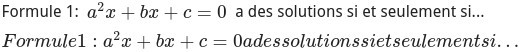
\includegraphics[scale=0.9]{gallery/whole_line.jpg}
    \caption[nom dans le sommaire]{Anomalie de rendu}
    \label{fig:gallery6}
\end{figure}

\paragraph{}
Il semble que MathJax essaye de faire un rendu de tout le texte contenu dans la ligne au lieu de simplement la formule. En regardant de plus près le contenu de la marque il s'avère qu'elle prenait effectivement toute le texte de la ligne en considération.
\paragraph{}
Pour pallier ce problème j'ai donc créé une fonction pour récupérer dans une marque les éléments du texte répondant aux expressions "\$ ... \$" ou "\$\$ ... \$\$". Ainsi, on passe à MathJax la formule au lieu du texte contenu dans la marque.
\paragraph{}
Pour le cas où l'utilisateur soit en train d'ajouter une formule à une ligne en contenant déjà une (imaginer que le texte est "\$ formule 1 \$ \$"), cet algorithme considère que les deux derniers dollars constituent une formule. Cela entraîne des problèmes de rendus qui sont très perturbants pour l'utilisateur en train rédiger. Pour pallier ce problème j'ai donc empêché le rafraîchissement d'une ligne contenant un nombre impair de \$.\\

\subsubsection{Doublons de marques : décalage des rendus}
\paragraph{}
Encore pendant que je travaillais sur une autre issue, j'ai remarqué un décalage dans les rendus MathJax. Par exemple : si sur la ligne 1 se trouvent les formules A et B, sur la ligne 2 la formule C et que l'utilisateur focus la formule B, alors sur la ligne 2 on verra s'afficher le rendu de la formule B. Ce décalage n'est pas transmis aux autres collaborateurs.
\paragraph{}
Il s'avère que si sur une ligne il y a deux formules, chacune de ces formules va générer une marque. On aura donc deux marques aux contenus identiques. Ainsi, quand la formule B est 'cassée', la marque de la formule A subsiste. Comme on extrait les formules depuis les marques, et comme on itère sur les marques et les jaxs en parallèle, on applique donc à la formule C le rendu de la formule B.
\paragraph{}
Pour pallier ceci j'ai repensé mon code pour pouvoir isoler la ligne contenant une formule en train d'être éditée pour pouvoir toujours garder synchronisés la liste des marques et la liste des jaxs. Toujours en itérant sur les marques, on compte le nombre de formules qu'elle contient :\\
\begin{itemize}
    \item S'il est égal à un, nous sommes dans un cas disons classique, et nous allons juste faire le rendu. Pour être sûr de mettre à jour la bonne jax par rapport à la liste des marques, on met en place un compteur symbolisant index de la prochaine jax à mettre à jour.
    \item S'il y a plusieurs formules dans cette marque, on stocke ce nombre et on passe à la marque suivante :\\
    \begin{itemize}
        \item Si la marque est différente et qu'on n'a pas passé autant de marques que le nombre de formules détectées, c'est que l'une d'elle est en édition. On ne met rien à jour et on augmente le compteur de la prochaine jax à mettre à jour.
        \item Si la marque est identique mais qu'on n'a pas passé autant de marques que de formules détectées alors on ne fait rien et on passe à la marque suivante.
        \item Si la marque est identique et qu'on a passé le bon nombre de marques alors aucune des formules n'est en train d'être éditée et on peut alors faire un rendu.
    \end{itemize}
\end{itemize}

\subsubsection{Limites}
\paragraph{}
Cette problématique a elle seule aurait dû constituer une issue plus importante que simplement une issue avec le label 'bug'. Cependant je devais aussi avancer sur d'autres fonctionnalités donc mon travail n'est pas aussi complet que ce que je l'aurai souhaité. Par exemple, la solution mise en place actuellement bloque le rendu des jaxs des lignes contenant un nombre impair de '\$'. Or il est possible que ce cas subvienne. Néanmoins, la mise à jour des formules est toujours possible si on focus la formule.
\paragraph{}
L'utilisation de MathJax a montré quelques difficultés lors d'un test réalisé avec neuf navigateurs. Des fois les formules disparaissaient complètement. Il est difficile de reproduire les scénarios où MathJax a dysfonctionné.
\paragraph{}
Avec un intervalle de cent millisecondes, il arrivait des fois que toutes les formules s'affichent en deux fois si on cassait/reformait les marques trop vite. Ce bug ne touche pas aux marques et disparaissait très rapidement. Pour régler le problème, l'intervalle est de maintenant trois secondes. Si cela sacrifie un peu le caractère 'temps-réel' cela offrira peut-être une meilleure stabilité au fonctionnement de MathJax en collaboration.

\newpage
\subsection{Création d'antisèches}
\paragraph{}
Afin d'améliorer l'expérience des utilisateurs de MUTE, deux issues ont été créées pour ajouter des cheat-sheets à l'éditeur, littéralement des antisèches. Ces antisèches contiendraient des rappels de syntaxe pour Markdown et MathJax. Nous avons décidé avec mon maître de stage que ces éléments seraient incrustés à droite du document, au même niveau que les informations le concernant (localisation du stockage et collaborateurs), afin que l'utilisateur puisse les avoir à portée tout en gardant accès à l'éditeur. Il m'a été suggéré de réfléchir à une solution à base d'onglets que je pourrais donc intégrer au niveau du composant nommé très justement "right-side".
\paragraph{}
Via mes recherches pour la barre d'outils, je me suis souvenue qu'Angular Material proposait un module Tabs (onglets) \cite{tabs}. J'ai donc immédiatement travaillé sur cette solution. J'avais alors deux manières d'organiser les informations : soit avoir trois onglets (Details, Markdown, MathJax), soit avoir deux onglets (Details, Cheat-sheets) avec dans Cheat-sheets deux onglets (Markdown et MathJax). J'ai opté pour la deuxième solution, car trois onglets prenaient trop de place, le nom des onglets était tronqué. De plus cela fait plus de sens de stocker toutes les cheat-sheets dans un même onglet.\\

\subsubsection{Markdown Cheat-sheet}
\paragraph{}
Pour le contenu, et après avoir regardé des équivalents sur d'autres éditeurs, j'ai opté pour une disposition sur deux colonnes avec à gauche le rendu, à droite la syntaxe associée. L'idée que j'avais était d'avoir un rendu intuitif et raccord avec le reste de l'interface et les guidelines Angular.
\paragraph{}
J'ai tout d'abord essayé de travailler avec les tables HTML, mais le rendu était peu satisfaisant. Le fait de voir un tableau à cet endroit paraissait trop scolaire, le rendu était trop chargé.\\
Au hasard de mes essais, j'ai englobé le contenu dans un card, un autre composant Angular. Pour comprendre à quoi cela correspond, la zone d'édition du document, ressemblant beaucoup à feuille blanche, est un card. Le fait d'avoir fait ainsi m'a donné l'idée qu'il serait intéressant pour l'utilisateur de voir ce que le rendu donne sur le document. Ainsi, et pour donner de la structure à l'antisèche, j'ai mis le card en gris clair, puis y ait inséré six autres cards, eux en blanc. Chacun de ses cards représentera les catégories suivantes : les headers, les styles, les listes, les images, les liens et le code informatique. J'ai créé ces catégories en m'inspirant de cette cheat-sheet Markdown \cite{mdcheat}. Précédant chacun de ces cards, un titre en gris foncé, taille h2 permet de nommer chacune de ces catégories et sert de séparateur naturel entre chacun des cards.
\paragraph{}
Afin que les rendus soient fidèles à ce que génère HyperMD, j'ai eu l'idée d'importer la feuille CSS liée à HyperMD dans la feuille CSS du right-side. Ainsi, pour chaque texte auquel je voudrais appliquer le rendu HyperMD je n'aurai qu'à appeler la classe correspondante. Mais, pour certainement une bonne raison mais qui m'échappe, le style ne s'appliquait pas. Après plusieurs essais, j'ai décidé recréer des classes dans la feuille de style de right-side pour reproduire le rendu HyperMD.
Cette solution a marché mais cela a produit une duplication de code, il y a certainement moyen de faire autrement.
\paragraph{}
Après présentation à mon maître de stage, celui ci m'a suggéré que le fond gris clair soit de même couleur que l'arrière plan de l'application. Ainsi, les cards ressortent vraiment, sont à la même élévation que la zone d'édition et donnent un effet "post-it" qui est, je pense, vraiment parlant pour l'idée de mémo. L'utilisateur a donc une réelle idée du rendu que peut avoir ces différentes syntaxes.
\paragraph{}
Enfin, mon maître de stage a également suggéré que la cheat-sheet ait son propre composant Angular, sous-composant de right-side.\\

\subsubsection{MathJax Cheat-sheet}
\paragraph{}
Pour cette antisèche, je suis partie sur le même concept d'apparence et de structuration.
\paragraph{}
Dans un premier temps, mon maître de stage et moi-même désirions que les rendus des formules soient générés par MathJax. MathJax étant utilisé uniquement par HyperMD, je n'avais jamais eu besoin de l'importer au sein de notre projet. Cette tâche seule s'est étalée sur trois jours. Pour ne pas pas perdre trop de temps, en parallèle, je commençais de mettre en place le composant qui allait contenir l'antisèche. Finalement, après que mon maître de stage soit venu m'aider à mettre en place MathJax, nous avons constater qu'une particularité de MathJax était bloquante : en effet, MathJax charge les formules globalement, sur l'ensemble de l'interface. Plus précisément : la liste de 'jax' mentionnée en 3.6 est unique à l'application. Ainsi, les rendus se retrouvaient décalés : la première formule dans l'éditeur avait son rendu dans l'antisèche, et toutes les autres formules se trouvaient décalée d'un cran.
\paragraph{}
Nous avons donc conclu qu'il serait plus simple que les rendus dans l'antisèche soient des images provenant d'impressions d'écrans. L'avantage à cela est que le rendu correspondra tout à fait à ce que MathJax produit dans l'éditeur, de plus, cela fait moins de formules à charger lors de l'affichage de l'antisèche.\\

\subsubsection{Inconvénients}
\paragraph{}
HyperMD prévoit que tout texte collé dans l'éditeur à partir du presse-papier soit automatiquement échappé. Par exemple, *Hello world!* devient \textbackslash*Hello world!\textbackslash*. Il en va de même si l'utilisateur choisit de copier/coller la syntaxe d'un élément l'intéressant de l'antisèche vers l'éditeur. En soit ce n'est pas vraiment une mauvaise chose, car l'utilisateur pourra effectuer des manipulations avant d'enlever les caractères d'échappement et que le rendu ne se fasse. De plus les sections copiées ne sont pas très longues. Mais cela nécessite quand même une manipulation supplémentaire. Sans compter que pour des utilisateurs moins au fait de l'utilisation de l'éditeur cela peut poser un problème de compréhension.
\paragraph{}
Un autre inconvénient vient de l'utilisation des Tabs. Dans l'onglet Details se trouve l'affichage des contributeurs du projet. Il se trouve que le contenu de cet onglet refusait de prendre tout l'espace. Ainsi, le contenu était réduit à un très petit espace, qui, par conséquent, générait une barre de défilement, ce qui n'était pas très esthétique. Mon maître de stage a pris en charge la résolution de ce problème. Cela a eu un effet sur les antisèches, qui ne sont plus contenues dans un card gris, mais sont juste disposées sur le fond de l'application. Le résultat reste très sensiblement le même.
\paragraph{}
Le dernier inconvénient vient de la manière dont sont implémentées les Tabs d'Angular Materiel. La première fois que l'on décide de consulter les cheat-sheets, les deux sous-onglets se découvrent et l'on voit par défaut la cheat-sheet Markdown. Or, l'onglet Markdown n'est pas marqué comme étant sélectionné.

\begin{figure}[H]
    \centering
    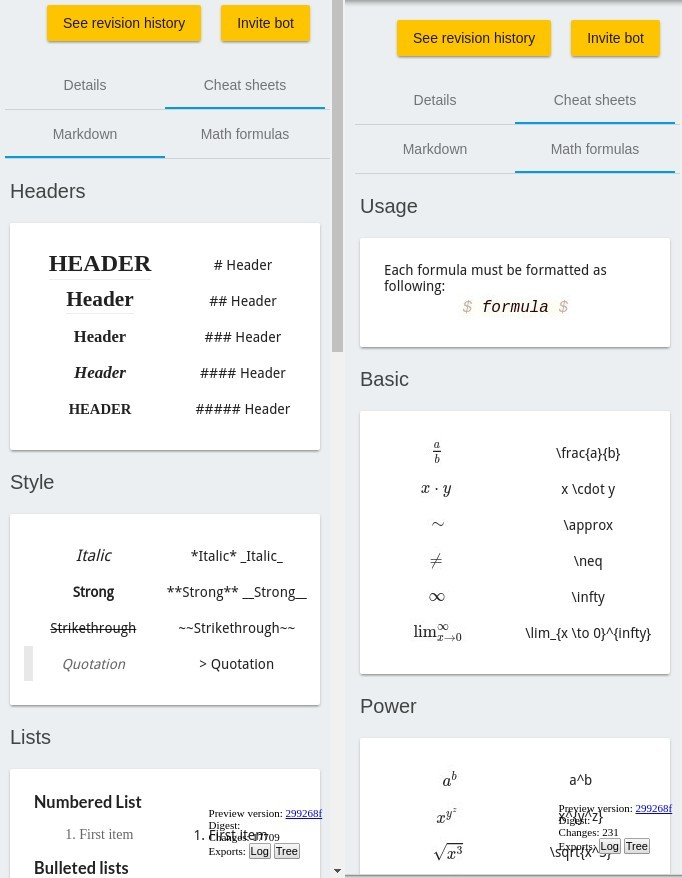
\includegraphics[scale=0.7]{gallery/cheat-sheets.jpg}
    \caption[nom dans le sommaire]{A gauche l'antisèche Markdown, à droite l'antisèche MathJax}
    \label{fig:gallery5}
\end{figure}


\newpage
\subsection{Tests}
\paragraph{}
Au cours du stage, il est arrivé que mon aide soit requise pour des tests. En effet, si l'on peut plus ou moins tester la robustesse de notre développement en ouvrant plusieurs navigateurs à la fois, il est impossible de reproduire l'édition simultanée d'un document par plusieurs collaborateurs. C'est pourquoi mon maître de stage, d'autres collègues, voire même moi-même demandions un coup de main à d'autres. Ces tests permettaient aussi que d'autres mettent en avant des scénarios où le développement de l'un ou de l'autre était incomplet.
\paragraph{}
De plus, avant que François Charoy décrète la fin du semestre et donc la fin des réunions hebdomadaires, chaque compte rendu de réunion était pris via MUTE. Nous pouvions ainsi tester la dernière démo, ce qui permettait de mettre en avant des oublis, des bugs ou des précisions sur les cas d'utilisations.\\

(Digest ?)

\newpage
\section{Bilan du stage}
\subsection{Avancement par rapport au cahier des charges prévu}
Si on se réfère au cahier des charges, la majorité des tâches a été accomplie. (tout fait à part EOP et exportation. que dire d'autre ?)

\subsection{Développement futur}
\subsubsection{Barre d'outil responsive}
Comme précisé dans la partie correspondante, la barre d'outil n'est pas responsive. Même s'il s'agit d'un détail, il reste toujours très apprécié et est un gage de qualité au sein d'une application.

\subsubsection{Attendre les nouvelles versions de certaines dépendances ?}
Certaines limites de développement évoquées dans ce rapport tiennent de la manière dont sont développées certaines librairies.

\paragraph{HyperMD}
Le projet HyperMD et MUTE présentaient une issue en commun : la création d'une barre d'outils. Au cours de mon analyse des fonctionnalités proposées par HyperMD j'ai dressé une liste des issues ouvertes sur ce projet et qui peut impacter le nôtre :
\begin{itemize}
    \item interprétation des paragraphes
    \item interprétation des tableaux
\end{itemize}
Après être entré en communication avec le propriétaire de ce projet il s'avère qu'HyperMD n'est pas sa priorité numéro une. Il conviendrait donc de traiter ces cas nous-mêmes.

\paragraph{MathJax}
Une particularité de cette librairie qui la rend unique face aux librairies utilisées dans MUTE est qu'elle est globale à l'application. Il serait préférable qu'on puisse la configurer pour la rendre globale à un document particulier. Depuis 2015, il est possible de voir sur le répertoire GitHub de ce projet qu'une version 3 est en cours de réflexion. Il semble donc qu'il se déroule une certaine période avant d'obtenir quelque chose de plus stable. Il serait peut-être envisageable de trouver une autre librairie qui remplisse les besoins escomptés.

\paragraph{Angular Material}
Au contraire de MathJax, le projet Angular Material semble plus actif. Il est donc très probables que les deux limites énoncées à l'encontre de l'utilisation d'Angular Material soient corrigées prochainement, mais elles représentent très certainement une priorité faible.

\subsubsection{Une nouvelle fonctionnalité : paramètres}
\paragraph{}
A l'issue de ce stage, beaucoup de nouvelles fonctionnalités ont été mises en place. Toujours soucieuse de l'expérience utilisateur, j'ai imaginé qu'il serait intéressant de mettre en place un système de paramétrage de certaines options.
\paragraph{}
Ainsi on pourrait laisser à l'utilisateur le soin de pouvoir activer/désactiver la barre d'outils, et les previews MathJax. Mais aussi, quand beaucoup de formules sont chargées au sein d'un même document, si la configuration de l'ordinateur de l'utilisateur met en cause le bon fonctionnement de MUTE, demander à augmenter l'intervalle de rafraîchissement des formules. Dans le même soucis de performances, s'il y a beaucoup de collaborateurs sur le même document, ou tout simplement par confort, animer le curseur d'un collaborateur seulement quand il écrit, voire complètement les désactiver.
\paragraph{}
Pour mettre en place cette fonctionnalité, on pourrait mettre en place un bouton paramètres dans le menu gauche de MUTE. Ce bouton pourrait faire apparaître une boîte de dialogue comportant la liste des différents paramètres cités précédemment. En face de ces éléments, on pourra mettre en place un objet d'Angular Material. Pour les activations/désactivations, des slige toogles \cite{slide}. Pour régler la fréquence des rafraîchissements et la complexité des animations, des sliders \cite{slider}.\\

\subsubsection{Améliorations des appels à MathJax}
\paragraph{}
En attendant une version plus stable de MathJax, et si aucune autre librairie viendrait à se substituer à celle-ci, nous avons discuté avec mon maître de stage de certaines dispositions qui pourraient être mises en place pour limiter son dysfonctionnement.
\paragraph{}
Dans un premier temps, il serait possible de ne plus demander le rendu des formules selon un intervalle de temps mais seulement quand une modification est perçue. S'il m'était possible de pouvoir détecter une modification, je n'ai cependant pas eu l'idée de comment faire "sortir" cette information d'HyperMD et de la transmettre à MUTE.
\paragraph{}
Grâce à l'API Netflux, il est possible d'ajouter au réseau pair-à-pair un "bot". L'idée première de cette fonctionnalité est de permettre à un utilisateur de pouvoir stocker son document sur la base de données OVH (où est hébergé MUTE) en plus de la base de données native du navigateur internet. Ce bot est relié à tous les autres pairs et peut aussi servir à faire des calculs qu'on lui aurait délégué. Ainsi, il serait possible de déléguer le rendu des formules MathJax à ce bot qui n'aurait plus qu'à transmettre le résultat aux autre pairs. Ainsi, les navigateurs pourraient s'affranchir de toutes ces requêtes MathJax.
\paragraph{}
Il en va sans dire que s'il était possible d'associer ces deux dispositions, on obtiendrait une utilisation moins prenante en ressources et certainement plus stable.\\

\subsection{Devenir de MUTE}
Coming soon...

\newpage
\addcontentsline{toc}{section}{Conclusion}
\section*{Conclusion}
Coming soon...

\newpage
\printbibliography[heading=bibintoc,title={Webographie}]

\newpage
\addcontentsline{toc}{section}{Glossaire}
\section*{Glossaire}

\clearpage

\newpage
\addcontentsline{toc}{section}{Annexes}
\section*{Annexes}

\newpage
\section*{Mots-clefs :}
\textbf{MUTE, collaborative-editing, rich-text-editor}

\end{document}